\chapter{Methode}
\section{De fietssimulatie}
Er wordt een simulatie gemaakt die de toestand van de fiets zo goed mogelijk probeert te benaderen. Er zal geen rekening gehouden worden met het manoeuvreren van de fiets of van tegenwind. Enkel de relevante meetwaarden worden bijgehouden. De simulatie is geparametriseerd om eenvoudig verschillende scenario’s te testen.
\\\\
Het voordeel van de fietssimulatie is de enorme flexibiliteit. Uren aan data kunnen in een moment tijd gegenereerd worden, waardoor het makkelijk is om verschillende tests uit te voeren. Hiervoor moeten slechts enkele instellingen aangepast worden. Het is ook mogelijk om slechts een enkele parameter aan te passen tijdens tests terwijl de rest constant blijft (\textit{ceteris paribus}), wat praktisch onmogelijk is in een veldtest. Omdat de simulatie bovendien een duidelijke referentie genereert voor de FCC (output van het fietsersmodel), kan de performantie van de cadanscontroller op een kwantitatieve manier worden geëvalueerd. Tijdens een veldtest zou de fietser alleen kwalitatief kunnen aangeven of hij of zij de voorspelde cadans goed vind. 
\section{Modelleren van het fietserkoppel}
Het fietserkoppel wordt gemodelleerd als een sinusfunctie met twee pieken per omwenteling van de trapas (2 benen), met het DC koppel van de fietser als parameter.
\\
\begin{gather*}
 T_{cy} = \gls{t_dc}(1+sin(2\theta_{cr}-\frac{\pi}{6}))
\end{gather*}
\\
Uit deze formule is het ook meteen duidelijk dat het DC koppel ook het vermogen-equivalent koppel is. Dat wil zeggen dat het DC koppel gedurende een volledige omwenteling van de trapas evenveel arbeid levert als het fietserkoppel.
\\
\begin{align*}
\int_{0}^{2\pi} T_{cy}(1+sin(2x-\frac{\pi}{6})) dx &= T_{cy} \int_{0}^{2\pi}(1+sin(2x-\frac{\pi}{6})) dx\\
&= T_{cy} \left[x-\frac{1}{2}sin(\frac{1}{3}(6x+\pi))\right]_0^{2\pi}\\
&= 2\pi \ T_{cy}
\end{align*}
\\
\noindent
Het gemiddelde koppel geleverd door de fietser wordt gemodelleerd als een proportionele regelaar. Het doel is om een bepaalde snelheid, $v_{ref}$, te behalen. Hoe groter het verschil is tussen de referentie snelheid en de eigenlijke snelheid, hoe meer kracht er geleverd zal worden. Als deze referentie snelheid overschreden wordt, dan zal er geen koppel meer geleverd worden. Dit wordt ook wel freewheelen genoemd. Om de kracht van de actor te limiteren, wordt er een maximum koppel ingesteld ($T_{dc,max}$) naar gelang de huidige cadans (\gls{omega_cr}). Zo wordt er meer kracht geleverd wanneer de cadans laag is, net zoals in de werkelijkheid. \gls{k} bepaalt de agressiviteit van de regelaar. De formules zien er als volgt uit:

\begin{gather*}
\gls{t_dc_max} = \frac{-\omega_{cr}}{2}+60 \tab (Figuur\ \ref{fig:koppeltoerentalkarakteristiek}) \\
T_{dc} = min(T_{dc,max},max(0,-K*(v_{bike}-v_{ref}))
\end{gather*}
\\
\begin{figure}
  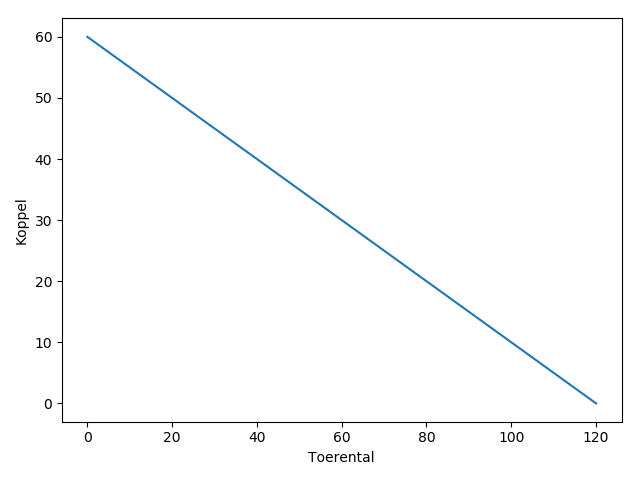
\includegraphics[width=\linewidth]{images/koppel-toerentalkarakteristiek.png}
  \caption{Het koppel-toerentalkarakteristiek}
  \label{fig:koppeltoerentalkarakteristiek}
\end{figure}
\\
\noindent Figuren \ref{fig:menselijkkoppelverloop} en \ref{fig:gesimuleerdkoppelverloop} tonen een menselijk koppelverloop en gesimuleerd koppelverloop, gesampled aan 10Hz. Zoals te zien is het gesimuleerde koppel heel consistent. Het menselijk koppel volgt duidelijk een cyclische functie, maar toont vormen van inconsistentie. Merk wel op dat er telkens een afwisseling is van een hoge en een lage piek. Dit wijst op een dominant been. Figuur \ref{fig:gesimuleerde koppel dominant been} toont een gesimuleerd koppelverloop van een fietser met een dominant been.
\\\\
\begin{figure}[t!]
\centering
\begin{subfigure}{.5\textwidth}
  \centering
  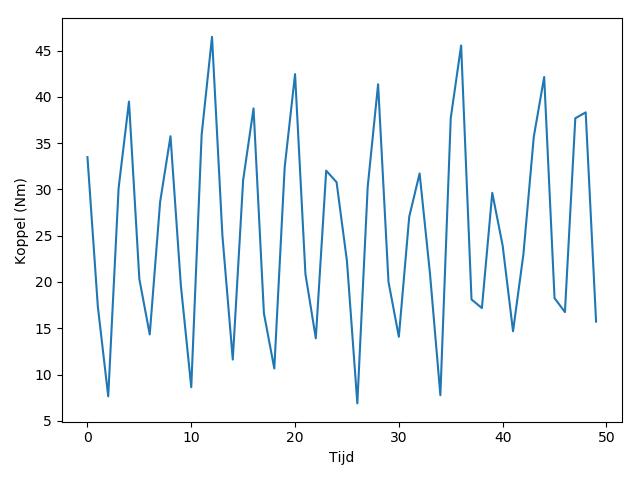
\includegraphics[width=\linewidth]{images/menselijkkoppel.png}
  \caption{Menselijk koppelverloop}
  \label{fig:menselijkkoppelverloop}
\end{subfigure}%
\begin{subfigure}{.5\textwidth}
  \centering
  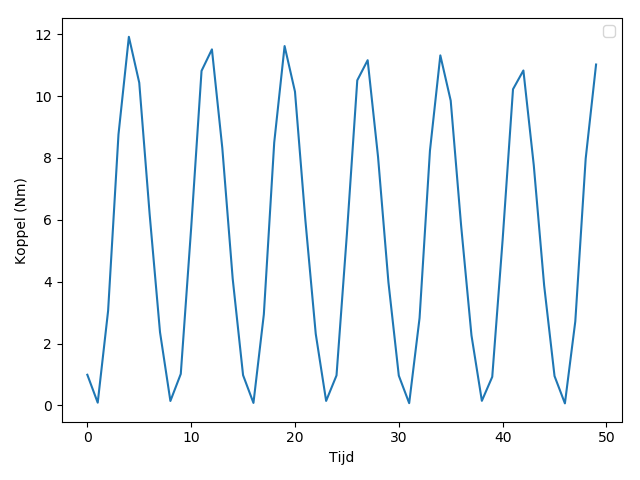
\includegraphics[width=\linewidth]{images/gesimuleerdekoppel.png}
  \caption{Gesimuleerd koppelverloop}
  \label{fig:gesimuleerdkoppelverloop}
\end{subfigure}
\begin{subfigure}{.5\textwidth}
  \centering
  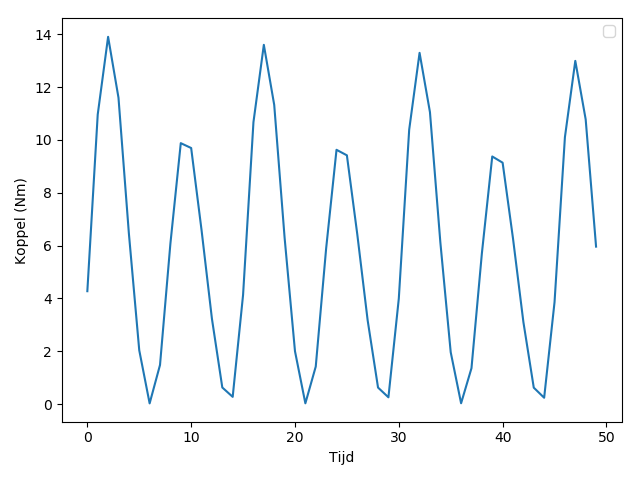
\includegraphics[width=\linewidth]{images/gesimuleerdekoppeldominantbeen.png}
  \caption{Gesimuleerd koppelverloop met dominant been}
  \label{fig:gesimuleerde koppel dominant been}
\end{subfigure}
\caption{Het koppelverloop van een mens (linksboven), de simulatie (rechtsboven) en een gesimuleerd dominant been (onderaan)}
\label{fig:koppelverloop mens-simulatie}
\end{figure}
\newpage
\begin{wrapfigure}{R}{0.5\textwidth}
  \centering
  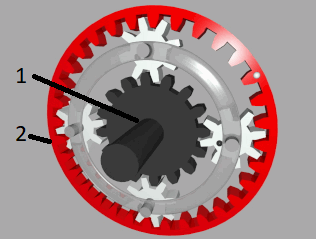
\includegraphics[width=\linewidth]{images/planeetwielmechanisme.png}
  \caption{Planeetwielmechanisme (bron: wikipedia)}
  \label{fig:planeetwielmechanisme}
\end{wrapfigure}

\noindent $T_{cy}$ is het koppel op de trapas. Dit moet nog overgebracht worden op het achterwiel. CoSaR maakt gebruik van een planeetwielmechanisme (figuur \ref{fig:planeetwielmechanisme}). Dit mechanisme laat toe om een grote overbrengingsverhouding te voorzien in een kleine ruimte. Het achterwiel-koppel wordt beïnvloed door het aantal tanden op het zonnewiel (1; \gls{ns}) en het ringwiel (2; \gls{nr}) en de overbrengingsverhouding tussen de trapas en het ringwiel (\gls{k_cr,r}). Het koppel op het achterwiel (\gls{t_rw}) ziet er als volgt uit:
\begin{gather*}
T_{rw}=T_{cy}*k_{cr,r}*\frac{nr+ns}{nr}
\end{gather*}
\\\\
Bovenop het vermogen geproduceerd door de fietser, levert CoSaR extra ondersteuning a.d.h.v. een motor (\gls{t_mg2}) gekoppeld aan het voorwiel. De fietser kan zelf een ondersteuningsniveau (\gls{s}) instellen tussen 0 en 5. Hoe hoger dit ondersteuningsniveau, hoe minder inspanning de fietser moet leveren. 
\begin{gather*}
T_{MG2}=min(35,S\thinspace .\thinspace T_{cy})
\end{gather*}

\section{Het fietsersmodel}
Hoe kiest een fietser zijn cadans? Dit is voor elke fietser verschillend en er is nog nauwelijks onderzoek naar gebeurd. Wielrenners trainen om sneller te kunnen trappen omdat dit efficiënter is. Ze kunnen een gemiddeld vermogen leveren van 300 Watt. De doorsnee fietser levert gemiddeld ongeveer 75 Watt tijdens een normale fietstocht. Het fietsersmodel zal hierop worden afgesteld, aangezien wielrenners niet de voornaamste doelgroep zijn voor CoSaR.
\\\\
Het fietsersmodel is een functie die op verschillende manieren uitgedrukt kan worden: op basis van de helling, gemiddeld koppel, of snelheid. Wat het correcte model is wordt in deze thesis niet uitgewerkt. Het is vooral van belang dat de cadanscontroller het model zo snel en zo nauwkeurig mogelijk kan achterhalen, ongeacht wat het model precies is. Hier wordt de volgende aanname gemaakt: hoe hoger het koppel geleverd door de fietser, hoe hoger de gewenste cadans. Wanneer de fietser bijvoorbeeld een helling oprijdt schakelt hij of zij een versnelling omlaag zodat de kracht die op de pedalen gezet moet worden aangenaam blijft. We stellen hier volgende eenvoudige modellen voor:
\begin{align*}
Gemiddeld \ koppel:\tab fcc &= \gls{f_k} . T_{dc}\\
Helling:\tab fcc &= \gls{f_h} . \alpha\\
Snelheid:\tab fcc &= \gls{f_v} . v_{bike}
\end{align*}
Er wordt verder aangenomen dat de fietser ook een zeker lineariteit verwacht bij lage snelheden. Dat wil zeggen dat een fietser het niet comfortabel vindt wanneer hij of zij snel moet trappen wanneer de fiets nog stilstaat of heel traag rijdt, ook al moet er op dat moment veel koppel geleverd worden om te kunnen vertrekken. Daarom wordt bij lage snelheden de FCC begrensd door een lineair oplopend maximum, te vergelijken met een mechanische fietsversnelling. Omdat de doorsnee fietser niet heel traag of heel snel trapt wordt de FCC begrensd tussen de 40 en 120 rpm.
\begin{figure}
  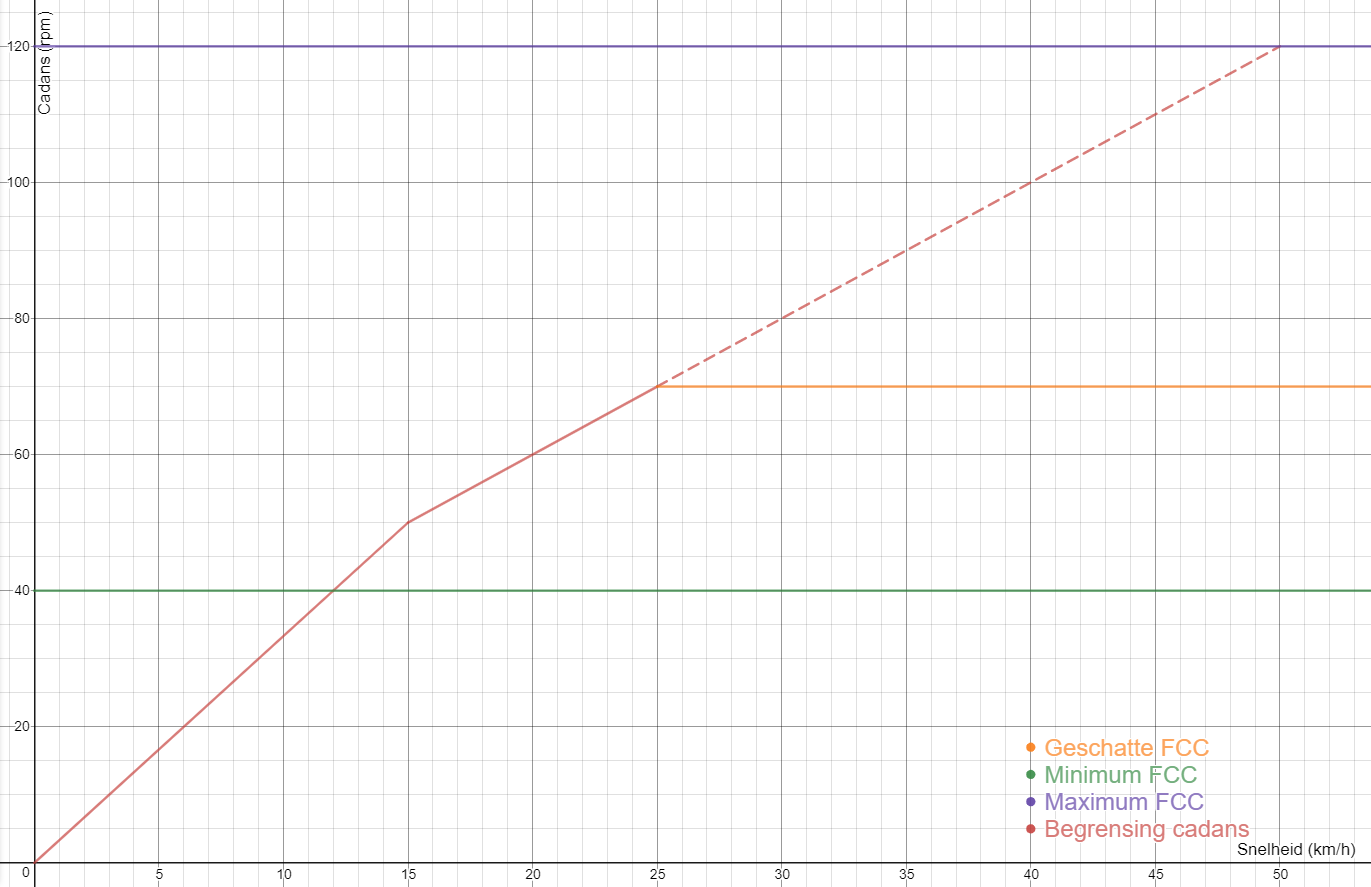
\includegraphics[width=\linewidth]{images/cadansverloop.png}
  \caption{Verwacht cadansverloop in functie van de snelheid.}
  \label{fig:cadansverloop}
\end{figure}
\newpage
\section{Het lastmodel}
De simulatie is voorzien van een lastmodel. Zoals in realiteit, werken lasten in op de fiets. Zwaartekracht, wrijving met de weg en luchtweerstand zijn gemodelleerd als volgt:
\\
\begin{align*}
\gls{f_grav}&=\gls{m} \ . \ \gls{g} \ . \ sin \ \alpha \\
\gls{f_friction}&=m \ . \ g \ . \ \gls{c_r} \ . \ cos \ \alpha \\
\gls{f_aero}&=\frac{\gls{c_d} \ . \ \gls{rho_aero} \ . \ \gls{a_aero} \ . \ v_{bike}^2}{2}
\end{align*}
Samen vormen ze de totale belasting op de fiets.
\[\gls{f_load} = F_{grav}+F_{friction}+F_{aero}\]
Deze lasten zorgen ervoor dat de simulatie een realistische hoeveelheid vermogen nodig heeft om een bepaalde snelheid te halen. Er wordt hier geen rekening gehouden met de wind. Ten eerste zou dit extra complexiteit toevoegen aan de simulatie. En ten tweede vermoeden we volgende hypothese:
\\\\
\tab De freely chosen cadence hangt af van de hoeveelheid last, van welke bron dan \tab ook, die de gebruiker ondervindt en de gebruiker zelf.
\\\\
Het voorgestelde lastmodel omvat deze vereiste. Door de helling en referentie snelheid te variëren ondergaat de fietser een veranderende last. Zoals in de realiteit zoeken mensen een bepaalde snelheid te halen. Wanneer de fietser een te hoge last ondervindt, bijvoorbeeld door een berg op te rijden, moet hij of zij meer vermogen genereren om zijn of haar gewenste snelheid te behouden. Hiervoor zijn 2 mogelijkheden: het verhogen van het koppel of de trapsnelheid. Mensen zijn meer geneigd om hun gewenste cadans te behouden, ongeacht het koppel (binnen bepaalde grenzen). De formule voor mechanisch vermogen gaat als volgt:
\[\gls{p}=T_{cy} \ . \omega_{cr} \]
Om het lastmodel correct te laten werken, moet er nog een helling gegenereerd worden. Om veel werk uit te sparen met het uitstippelen van parcours, wordt dit dynamisch gegenereerd met behulp van perlin noise. Perlin noise kan gebruikt worden om willekeurige getallen te genereren waarbij opeenvolgende getallen weinig van elkaar verschillen. Een perfecte kandidaat dus om terrein te simuleren. Om verschillende trajecten te creëren, kan de seed variabele aangepast worden. Een hellingsgraad wordt in de fietswereld vaak percentueel voorgesteld. Deze implementatie heeft echter radialen nodig. De helling zal beperkt worden tussen $\approx$ 0 en 10\% (0 en 0.1 radialen). Ter vergelijking, de Koppenberg heeft een gemiddeld stijgingspercentage van 11.6\%. Het minimum stijgingspercentage is zo gekozen dat de simulatie zo weinig mogelijk gaat freewheelen.
\begin{figure}[t]
  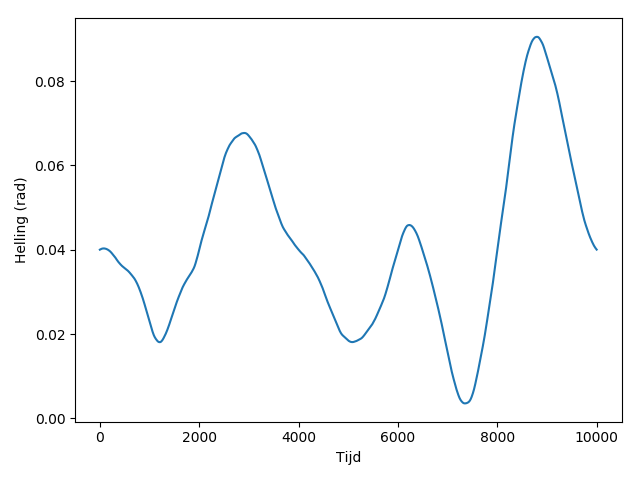
\includegraphics[width=\linewidth]{images/parcour_slope_example.png}
  \caption{Voorbeeld helling verloop}
  \label{fig:hellingverloop}
\end{figure}
\newpage
\section{Snelheidsvergelijking}
\noindent De snelheid wordt berekend met een standaardformule: vorige snelheid plus acceleratie met respect tot de genomen tijdsprong. De acceleratie is in functie van de last, het totaalgewicht (m), het vermogen geleverd door de fietser op het achterwiel ($T_{rw}$) en het vermogen van een motor bevestigd op het voorwiel ($T_{MG2}$). 
\\\\
De bewegingsvergelijking van de fiets is, met inbegrip van het lastmodel en het fietsersmodel:
\[F \ = \  m \ . \ a \]
Deze vergelijking wordt elke tijdsstap geïntegreerd met behulp van een voorwaartse Euler methode:
\[F = m.(\frac{v_{bike}[h]-v_{bike}[h-1]}{\Delta t})\]
\[ \frac{\Delta t. F}{m}=v_{bike}[h]-v_{bike}[h-1]\]
\[v_{bike}[h]=v_{bike}[h-1]+\Delta t .\frac{1}{m}.F\]
\[v_{bike}[h] \ = \ v_{bike}[h-1] \ + \Delta t  \ . \frac{1}{m} \ . \ (\frac{T_{MG2} \ + \ T_{rw}}{r_w} \ - \ F_{load})\]
De volledige simulatie ziet er als volgt uit:
\\\\
 \fbox{\begin{minipage}{\linewidth}
for h in 1..$\#$tijdssprongen\\
\tab $T_{dc,max} = \frac{-\omega_{cr}[h-1]}{2}+60$\\
\tab $T_{dc} = min(T_{dc,max}, \ max(0,-K*(v_{bike}[h-1]-v_{ref}))$\\
\tab $fcc = f(T_{dc})$\\
\tab $\omega_{cr}=cadans(v_{bike}[h-1], \ T_{dc}, \ fcc)$\\
\tab $\theta_{cr}=\theta_{cr}[h-1] + \Delta t \ . \ \omega_{cr}$ \\
\tab $T_{cy} = T_{dc}(1+sin(2\theta_{cr}-\frac{\pi}{6}))$\\
\tab $T_{rw}=T_{cy}*k_{cr,r}*\frac{nr+ns}{nr}$\\
\tab $T_{MG2}=min(35, \ S \ . \ T_{cy})$\\
\tab $F_{grav}=m \ . \ g \ . \ sin \ \alpha$\\
\tab $F_{friction}=m \ . \ g. \ c_r \ . \ cos \ \alpha$\\
\tab $F_{aero}=\frac{c_d \ . \ \rho_{aero} \ . \ A_{aero} \ . \ v_{bike}[h-1]^2}{2}$\\
\tab $F_{load} = F_{grav}+F_{friction}+F_{aero}$\\
\tab $v_{bike} \ = \ v_{bike}[h-1] \ + \Delta t  \ . \frac{1}{m} \ . \ (\frac{T_{MG2} \ + \ T_{rw}}{\gls{r_w}} \ - \ F_{load})$
\end{minipage}}

\section{On-line voorspellen van de cadans}
Een groot deel van de toestand van de fiets wordt berekend. Om een efficiënt algoritme te creëren moet enkel de relevante data bekeken worden. Zo worden de volgende attributen gebruikt: snelheid, koppel, hoek van de trapas en helling. 
\\

\begin{wrapfigure}{R}{0.40\textwidth}
  \centering
  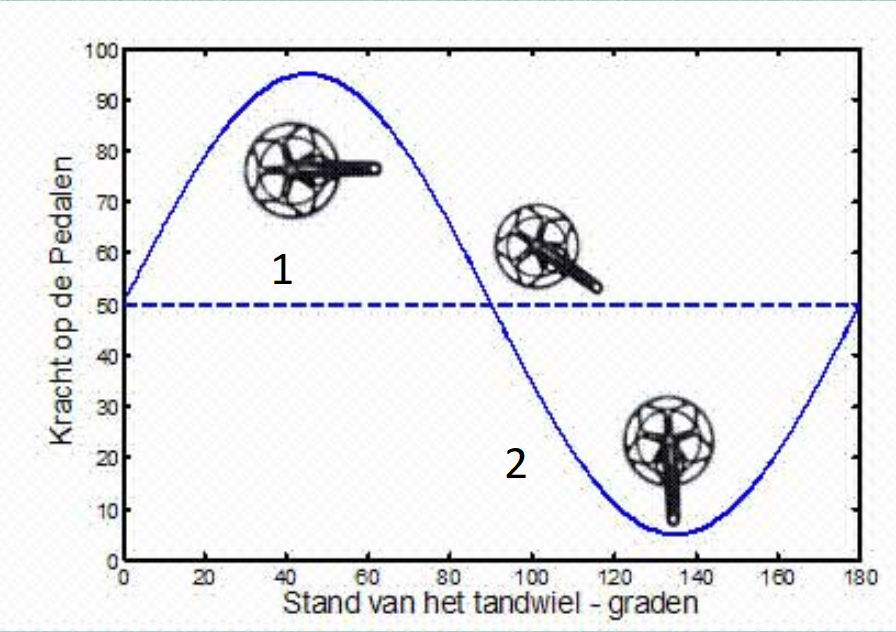
\includegraphics[width=\linewidth]{images/trapcyclus.png}
  \caption{Evolutie koppel in functie van hoek trapas}
  \label{fig:Evolutie koppel in functie van hoek trapas}
\end{wrapfigure}
\noindent De helling is vanzelfsprekend. Dit is de voornaamste vorm van last en zal dus een impact hebben op de freely chosen cadence van de fietser. De hoek van de trapas op zich heeft niet veel betekenis. En enkel het koppel ook niet. Er kan bijvoorbeeld een koppel geleverd worden van 20Nm. Dit koppel kan op verschillende plaatsen geleverd worden in de trapcyclus. Als dit in de situatie 2 geleverd wordt, dan is dit waarschijnlijk het laagste koppel in de trapcyclus. Wordt dit geleverd gedurende de neergaande beweging (1), dan is dit het hoogste koppel. Deze verschillende situaties zullen een verschillende cadans nodig hebben. Tijdens de eerst situatie wordt er gemiddeld meer koppel geleverd, wat wijst op een grote last. Dus verwachten we hier een hoge cadans. De tweede situatie daarentegen zal gemiddeld een lagere last hebben. Daarom wordt in conjunctie met het koppel de hoek van de trapas gebruikt. Snelheid is ook een relevant attribuut. In situaties met verschillende snelheden en dezelfde last gaat de cadans verschillen.
\newpage
\section{Preprocessing}
Niet elk algoritme heeft nood aan genormaliseerde input. Voor algoritmes die een afstandsfunctie gebruiken is standaardisatie cruciaal. De doelvariabele daarentegen moet niet genormaliseerd worden volgens Warren S. Sarle \cite{preprocessing faq}. In zijn FAQ schrijft hij dat het standaardiseren van de output voornamelijk voordelige effecten heeft op de initiële gewichten. Wanneer er meerdere doelvariabele zijn en als deze ver uit elkaar liggen, kan het wel nuttig zijn om deze te normaliseren. In dit geval is dat niet nodig aangezien enkel de cadans voorspeld zal worden.
\\\\
\noindent Ten eerste zal de data in sequentie gegoten worden. Een sequentie wordt gezien als een aantal vectoren ($x_t$) over verschillende tijdstippen. Een enkele data meting op zich is niet genoeg om een accurate voorspelling te maken, maar te veel data gebruiken is ook niet goed aangezien de voorspellingen tijdig moeten geleverd worden.
\\
\begin{gather*}
x_t = \begin{bmatrix} 
       \theta _{cr} \\ T_{cy,m} \\ v_{bike} \\ \alpha
     \end{bmatrix} \tab
sequentie = \begin{bmatrix} 
       x_t \\ x_{t-1} \\ ... \\ x_{t-n}
     \end{bmatrix} 
\end{gather*}
\\
\noindent Ten tweede zal de hoek van de trapas niet in zijn zuivere vorm gebruikt worden. De hoek van de trapas is een variabele tussen nul en twee pi. Het probleem hier is dat het begin en het einde van een cyclus ver uit elkaar liggen. Voor de mens is het evident dat nul en twee pi hetzelfde zijn, maar voor de computer is dit een groot verschil. Daarom zal de sinus en de cosinus van de hoek genomen worden zodat het begin en einde dicht bij elkaar liggen (figuur \ref{fig:preprocessing hoek trapas}). Zo leren we het algoritme bij dat de data zich cyclisch gedraagt.

\begin{figure}[h]
  \centering
  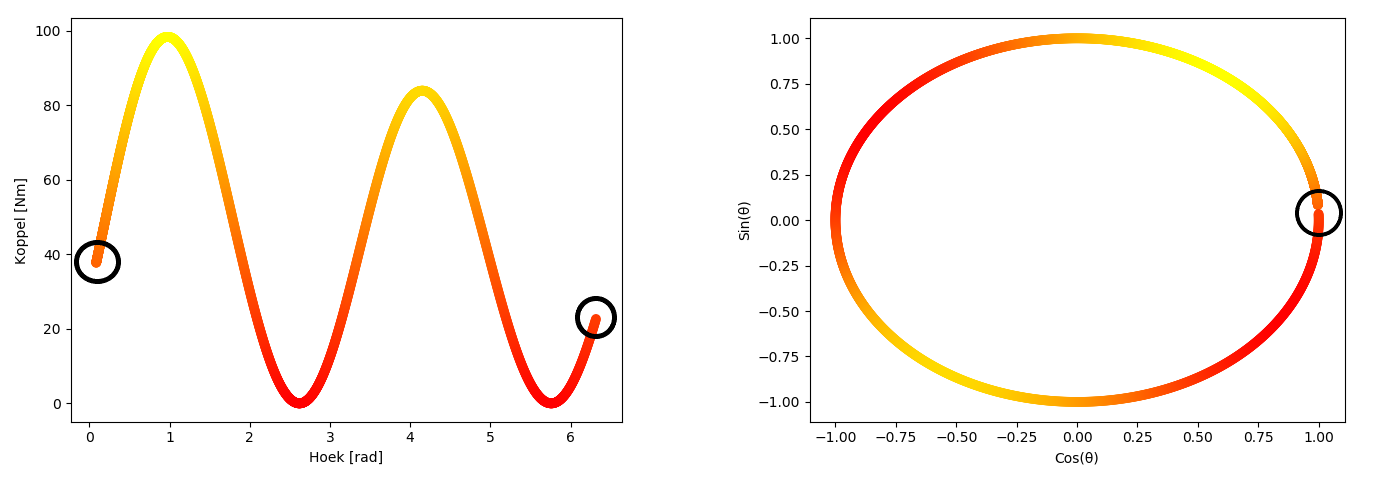
\includegraphics[width=\linewidth]{images/preprocessing-hoek.png}
  \caption{Figuur links toont dat het begin en einde van een trapcyclus ver uit elkaar liggen. Figuur rechts toont dat beide punten van de linkse figuur dicht bij elkaar liggen.}
  \label{fig:preprocessing hoek trapas}
\end{figure}

\noindent Ten slotte kan er ruis zitten op de metingen. Er zal altijd wel een klein foutje zitten op de data omdat de meetapparatuur niet perfect is. Het is mogelijk dat trillingen van de motor of het wegdek een impact kunnen hebben, voornamelijk op het geleverde koppel. Voor deze iteratie zal hier geen rekening mee gehouden worden. Ruis van het wegdek komt voor op een frequentie van ongeveer 20 Hz. Dit kan nog opgemerkt worden als er op voorhand data wordt gesampled op hogere frequentie. Ruis van de motoren daarentegen komt voor op 13000 Hz. Ver boven de gewilde sample frequentie en zal dus afgebeeld worden op lagere frequenties. Het huidige systeem zal geen rekening houden met beide soorten ruis. 

\begin{figure}[h]
  \centering
  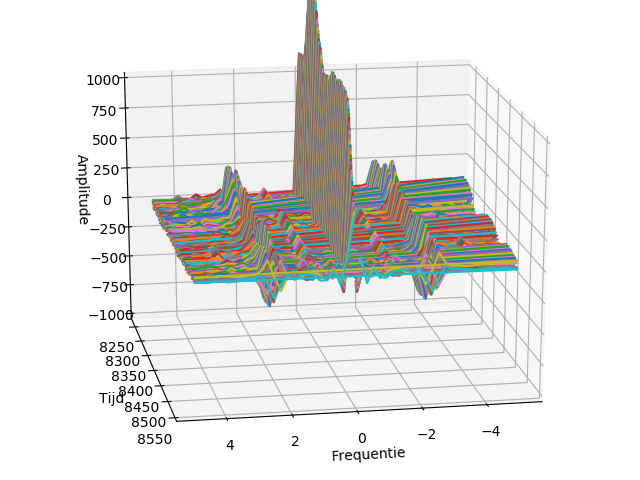
\includegraphics[width=\linewidth]{images/fft_fietser.png}
  \caption{Een Fast Fourier Transformatie van het menselijk koppelverloop.}
  \label{fig:preprocessing hoek trapas}
\end{figure}

\section{Algoritmes}
\subsection{Passive Aggressive Algorithm}
Het \gls{pa} algoritme, beschreven in de paper van Crammer et al. \cite{pa algorithm}, is een online algoritme gelijkaardig aan een perceptron. Net zoals de perceptron, doet PA de matrixvermenigvuldiging $y_t=w_t \cdot x_t$ om de voorspelling te berekenen. Het grootste verschil tussen beide is hoe de gewichten geüpdatet worden. Het PA algoritme is bruikbaar voor classificatie, regressie, uniclass voorspellingen en multiclass problemen.
\\\\
\noindent Het PA algoritme, zoals de naam weggeeft, kan zich zowel passief als agressief gedragen. Het trainen van PA bestaat uit twee stappen. In de eerste stap wordt er een voorspelling $y_{t,p}$ gemaakt a.d.h.v. de input vector $x_t$ en gewichtenmatrix $w$. Hierna wordt het echte label $y_t$ bekendgemaakt. Als de fout kleiner is dan een voorgedefinieerde waarde $\epsilon$, dan zullen de gewichten niet geüpdatet worden. Als de error toch groter is dan deze marge, dan zullen de gewichten $w$ aangepast worden zodat de fout voor de huidige instantie nul wordt. PA past de gewichten aan zodat het verschil tussen het vorige gewicht en het nieuwe gewicht minimaal is. 
\[
    loss_{\epsilon} (w_t;(x_t,y_t))=\left\{
                \begin{array}{ll}
                  0 \tab \tab \tab \ \ |w \cdot x - y| \leq \epsilon \\
                  |w \cdot x - y| - \epsilon \tab anderzijds
                \end{array}
              \right.\\
\]
\[
    w_{t+1}= \argmin_{w \in \mathbb{R}^n}
     \frac{1}{2}||w-w_t||^2 \tab zodat \ loss_{\epsilon} (w_{t+1};(x_t,y_t)) = 0
\]
Door de agressiviteit van het standaard PA algoritme kunnen er problemen ontstaan wanneer er veel ruis zit op de data. Daarom heeft Crammer et al. twee extra versies, PA-I en PA-II, gemaakt die dit probleem oplost. Beide versies voegen een slack variabele $\xi$ toe. Deze variabele zorgt ervoor dat bij het aanpassen van de gewichten, de fout kleiner of gelijk moet zijn aan $\xi$ in plaats van nul. Beide versies hebben ook een agressiviteits parameter C die deze $\xi$ beïnvloedt. Dit is een vorm van regularisatie om overfitting te voorkomen.

\[
   PA-I \tab w_{t+1}= \argmin_{w \in \mathbb{R}^n}
     \frac{1}{2}||w-w_t||^2 + C\xi \tab zodat \ loss_{\epsilon} (w_{t+1};(x_t,y_t)) \leq \xi
\]
\[
   PA-II \tab w_{t+1}= \argmin_{w \in \mathbb{R}^n}
     \frac{1}{2}||w-w_t||^2 + C\xi^2 \tab zodat \ loss_{\epsilon} (w_{t+1};(x_t,y_t)) \leq \xi
\]

De nieuwe gewichtenmatrix $w_{t+1}$ wordt als volgt berekent:
\[
w_{t+1}=w_t+ \tau_t y_t x_t
\]
\begin{align*}
\tau_t &= \frac{loss_t}{||x_t||^2} \tab \tab (PA)\\
\tau_t &= min \{ C, \frac{loss_t}{||x_t||^2} \} \ \ (PA-I)\\
\tau_t &= \frac{loss_t}{||x_t||^2+\frac{1}{2C}} \tab (PA-II) 
\end{align*}


\subsection{Decision Tree en Random Forest}
Een \gls{dt} is een rule-based model. Dit algoritme is snel (greedy), maar kan niet goed om met ruis. Dit model is gekend om makkelijk te overfitten. Daarom wordt het \gls{rf} algoritme simultaan bekeken.
\\\\
Een DT is een binaire boom. In elke knoop wordt een binair keuzepunt gemaakt op basis van een attribuut. Dit keuzepunt is gekozen zodat de data optimaal gesplitst is over beide takken. Sci-kit learn biedt de mogelijkheid aan om de maximum diepte van de boom te beperken. Wanneer deze parameter niet ingesteld is, zal de DT blijven groeien totdat alle blad nodes "puur" zijn. Een correcte diepte kiezen is een enorm moeilijke taak.
\\\\ 
RF is een ensemble. Dit wilt zeggen dat meerdere algoritmes, in dit geval meerdere DT’s, gebruikt worden om een betere voorspelling te maken. L. Breiman \cite{randomforest paper} beweert is zijn paper dat alle RF’s convergeren zodat overfitting geen probleem is. In tegenstelling tot DT’s, kiest een RF geen optimaal attribuut wanneer een node gesplitst wordt. De variabele worden at random gekozen, waardoor geen enkele boom dezelfde is. De verschillende bomen trainen niet met exact dezelfde trainingsdata. Ze passen Bootstrap Aggregating toe, of bagging. Dit houdt in dat uit de originele trainingsset data wordt gesampled at random. Een instantie kan meerdere keren gesampled worden. Deze techniek reduceert de variantie.
\section{Postprocessing}
De cadans variëert lichtjes doorheen een trapcyclus, zowel in het echt als in de simulatie. De voorspellingen zullen dezelfde trend vertonen. Bovendien kan een beetje ruis of het gedrag van de fietser voor afwijkingen zorgen, bijvoorbeeld een grote sprong tussen twee voorspellingen. Dit kan ergerend zijn voor de fietser.
\\\\
Dit probleem kan op verschillende manieren opgelost worden. Gebruikmakend van de huidige en vorige voorspellingen (\gls{fcc_pred}) of de vorige schatting ($FCC_{est}$). De vorige instelling is de cadans die is doorgegeven aan de fiets controller.
\begin{align*}
\gls{ma} \tab  FCC_{est,t} &= \frac{\sum_{i=0}^{n} FCC_{pred,t-i} }{n}\\
\gls{es} \tab FCC_{est,t} &= \gls{sf} . FCC_{pred,t} + (1-sf) . FCC_{est,t-1}
\end{align*}
MA lost beide problemen goed op. Meer voorspellingen leidt tot stabielere schattingen, maar dit introduceert een vertraging (lag) op de cadans. I.e. wanneer de omstandigheden veranderen, zal de ingestelde cadans slechts na enkele iteraties optimaal zijn, in plaats van onmiddellijk. ES verminderd de amplitude van de oscillaties slechts in mindere mate. De onderstaande figuren tonen wat de impact is van ES en MA op ruizige voorspellingen (20\% kans op ruis tussen -10 en +10).
\begin{figure}[t!]
\centering
\begin{subfigure}{.5\textwidth}
  \centering
  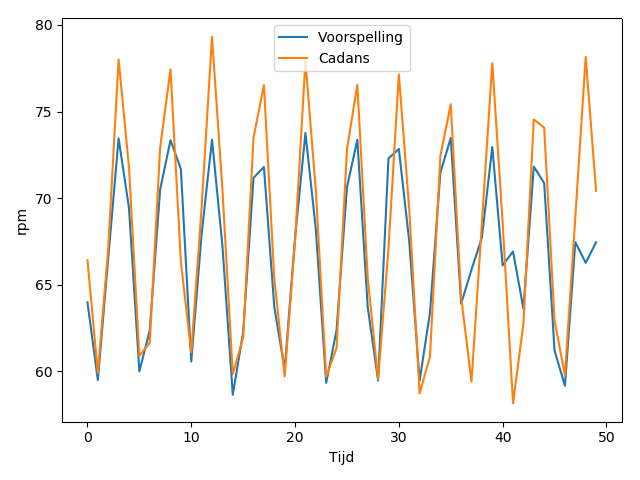
\includegraphics[width=\linewidth]{images/actual-prediction+noice,nopp.png}
  \caption{Geen postprocessing}
  \label{fig:geen postprocessing}
\end{subfigure}%
\begin{subfigure}{.5\textwidth}
  \centering
  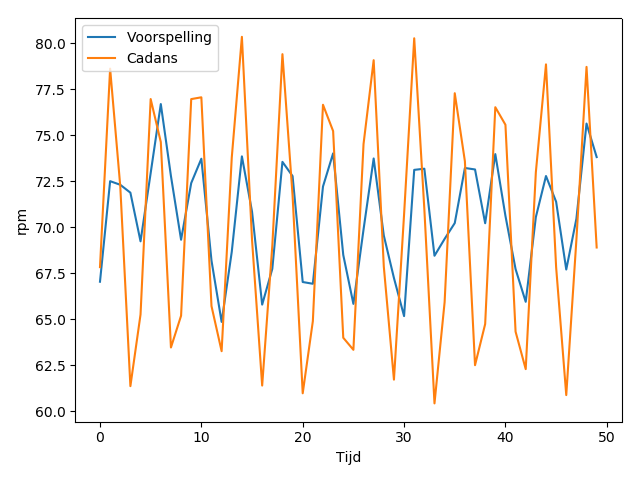
\includegraphics[width=\linewidth]{images/actual-prediction+noice,es.png}
  \caption{Exponential Smoothing}
  \label{fig:exponential smoothing postprocessing}
\end{subfigure}
\begin{subfigure}{.5\textwidth}
  \centering
  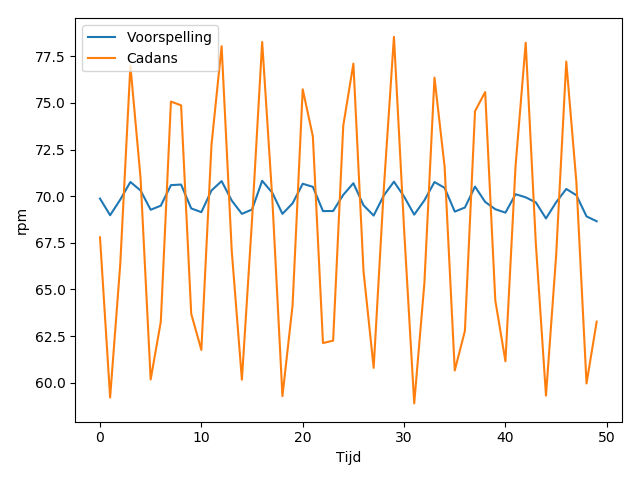
\includegraphics[width=\linewidth]{images/actual-prediction+noice,ma.png}
  \caption{Moving Average}
  \label{fig:moving average postprocessing}
\end{subfigure}
\caption{De effecten van verschillende postprocessing technieken.}
\label{fig:effecten postprocessing}
\end{figure}

